%%%%
%       _  _____  ___  _____  _   _  ___ 
%      / \|_   _||_ _||_   _|| | | |/ __|
%     / △ \ | |   | |   | |  | |_| |\__ \
%    /_/¯\_\|_|  |___|  |_|   \___/ |___/
%                 EDUCAÇÃO
%    Modelo de TCC - Ciência da Computação
%%%%

\documentclass[12pt]{article}

\usepackage{sbc-template}
\usepackage{graphicx, url}
\usepackage[utf8x]{inputenc}
\usepackage[brazil]{babel}
\usepackage[T1]{fontenc}
\usepackage[english=american]{csquotes}
\usepackage{float}
\usepackage{comment}
\usepackage{amsmath}
\usepackage{amssymb}
\usepackage{enumitem}
\usepackage{subcaption}
\usepackage{setspace}
\usepackage{listings}
\usepackage[scaled=0.85]{beramono}
\usepackage{tabularray}
\usepackage[hidelinks, breaklinks=true]{hyperref}
%\usepackage{hyperref}
%\hypersetup{
%    colorlinks=true,
%    allcolors=blue,
%}

% %%%%%%%%%%%%%%%%%%%%%%%%%%%%%%%%%%%%%%%%%%%%%%%%%%%%%%%%%%%%%%
% define o modelo de referencias
\usepackage[style=abnt, giveninits, uniquename=mininit, repeatfields]{biblatex}
\emergencystretch=1em

% indica o arquivo com as referencis bibliograficas
\addbibresource{sbc-template.bib}

% carrega o pacote com alterações para Computação Atitus
\usepackage{sty/cc_atitus}
% %%%%%%%%%%%%%%%%%%%%%%%%%%%%%%%%%%%%%%%%%%%%%%%%%%%%%%%%%%%%%%

% %%%%%%%%%%%%%%%%%%%%%%%%%%%%%%%%%%%%%%%%%%%%%%%%%%%%%%%%%%%%%%
% REFERENCIAS DEVERÃO SER INCLUÍDAS NO ARQUIVO: sbc-template.bib
%
% SOBRE CITAÇÕES:
% Para citar no padrão '(Autores, ano)' use: \cite{chave}
% Para citar no padrão 'Autores (ano)'  use: \textcite{chave} ou \citeonline{chave}
% Para citar no padrão 'Autores'        use: \citelastname{chave}
% Para citar no padrão 'Autor (ano), Autor (ano) e Autor (ano)' use: \textcites{chave1}{chave2}{chave3}
% Para citar no padrão '(Autor, 2009c; Outro Autor, 2009; Outro Autor, 2015)' use: 
%  \cites{chave1}{chave2}{chave3}
%  ou
%  \cite{chave1, chave2, chave3}

% Demais exemplos ver documento:
%  https://github.com/abntex/biblatex-abnt/raw/master/doc/biblatex-abnt.pdf
%
% Normas ABNT: https://usp.br/sddarquivos/arquivos/citacoes10520.pdf
%              https://usp.br/sddarquivos/arquivos/abnt6023.pdf
%              https://www.fct.unesp.br/Home/Biblioteca/abnt/abnt-atualizado-dez-2023.pdf
%
% %%%%%%%%%%%%%%%%%%%%%%%%%%%%%%%%%%%%%%%%%%%%%%%%%%%%%%%%%%%%%%
% Atualizações no modelo
% 2024-09-23: (fahadkalil) Ajuste para quebra automática de linhas nas células de uma tabela
% 2024-10-17: (fahadkalil) Inserção de comentários com outras citações e indicação de uso do comando "\enquote"
% 2025-06-05: (fahadkalil) Adição de novos exemplos de referências bibliográficas, figuras e tabelas / Correção para que campos desnecessários no arquivo .bib sejam ignorados na renderização / Correção de espaçamento no comando \begin{itemize} usando opções adicionais na seção Trabalhos Relacionados / Correção de recuos quando utilizado o comando \begin{description} / Correção na fonte e espaçamentos do comando 'lstlisting'
% %%%%%%%%%%%%%%%%%%%%%%%%%%%%%%%%%%%%%%%%%%%%%%%%%%%%%%%%%%%%%%
% CABEÇALHO
\title{Reescrita de Consultas SQL Baseada em Modelos de Linguagem de Grande Escala (LLM-based SQL Query Rewriting)} % titulo

\author{Luiz Eduardo Treméa\inst{1}, Fahad Kalil\inst{1}} % autor principal, orientador

\address{Ciência da Computação -- Atitus Educação\\
Passo Fundo -- RS -- Brasil
\email{1123471@atitus.edu.br, fahad.kalil@atitus.edu.br}
}
% %%%%%%%%%%%%%%%%%%%%%%%%%%%%%%%%%%%%%%%%%%%%%%%%%%%%%%%%%%%%%%

\begin{document}
\maketitle % Não remova essa linha!

\begin{abstract} % resumo em inglês
  Escreva seu resumo em língua estrangeira (inglês)...
\end{abstract}
     
\begin{resumo}
  Resumo do trabalho (português)...  
\end{resumo}

\section{Introdução}
Cenários, motivação, justificativa, problema de pesquisa, objetivo geral e específicos (taxonomia de Bloom);

\section{Referencial Teórico}

\subsection{Evolução da Otimização de Consultas e Uso de Inteligência Artificial}

A otimização de consultas em sistemas de gerenciamento de bancos de dados tem sido historicamente sustentada por três componentes centrais: a estimação de cardinalidade, o modelo de custo e a enumeração de planos. Nesse contexto, a qualidade do plano gerado depende diretamente da precisão das estimativas de volume de dados intermediários e da adequação da função de custo associada aos recursos computacionais.

Apesar de amplamente adotadas, essas abordagens apresentam limitações significativas em cenários contemporâneos, especialmente quando os dados apresentam correlações complexas entre atributos ou quando há variações frequentes na carga de trabalho. Nesses casos, erros de estimação podem comprometer a seleção do plano físico, resultando em degradação de desempenho \cite{marcus2019neo,marcus2021bao}.

Nesse contexto, surge o paradigma de \textit{Learned Query Optimization} (LQO), no qual técnicas de aprendizado de máquina são incorporadas ao processo de otimização. O sistema \textit{Neo} propõe um otimizador baseado em redes neurais profundas capaz de aprender padrões de execução a partir de consultas reais, adaptando-se dinamicamente ao comportamento dos dados \cite{marcus2019neo}. De forma complementar, o sistema \textit{Bao} introduz um mecanismo de otimização híbrida que utiliza aprendizado por reforço para fornecer sugestões de execução por consulta, melhorando o desempenho em cenários reais \cite{marcus2021bao}.

\subsection{Reescrita de Consultas SQL com Modelos de Linguagem}

A reescrita de consultas SQL tem como objetivo transformar uma consulta em outra semanticamente equivalente, porém mais eficiente do ponto de vista computacional. Diferentemente de abordagens de \textit{Text-to-SQL}, o foco da reescrita reside em modificar consultas já estruturadas, mantendo a equivalência lógica dos resultados.

O método \textit{LLM-R2} utiliza modelos de linguagem para sugerir regras de reescrita, combinando aprendizado contrastivo para aprimorar representações de consultas \cite{li2024llmr2}. De maneira semelhante, o sistema \textit{R-Bot} emprega uma abordagem baseada em recuperação de evidências estruturais e semânticas, com o objetivo de orientar o modelo e reduzir erros durante o processo de reescrita \cite{sun2025rbot}.

Além disso, o sistema \textit{QUITE} utiliza uma arquitetura baseada em múltiplos agentes que interagem por meio de um fluxo controlado, explorando estratégias de reescrita com realimentação do sistema de banco de dados \cite{song2025quite}. Já o sistema \textit{LITHE} propõe mecanismos adicionais para garantir a correção semântica das consultas geradas, incorporando validações baseadas em análise lógica e estatística \cite{dharwada2026lithe}.

\subsection{Estimativa de Cardinalidade e Modelos Aprendidos}

A estimação de cardinalidade é amplamente reconhecida como um dos principais fatores que influenciam a qualidade do plano de execução em sistemas de banco de dados, pois determina a previsão do volume de dados manipulados em cada etapa da execução da consulta.

O modelo \textit{NeuroCard} propõe um estimador baseado em redes neurais autorregressivas capaz de capturar correlações complexas entre múltiplas tabelas sem assumir independência entre atributos \cite{yang2021neurocard}. Por outro lado, o método \textit{FLAT} introduz um modelo gráfico que combina fatoração independente e condicional, buscando equilibrar precisão e eficiência computacional \cite{zhu2021flat}.

Essas abordagens evidenciam uma evolução significativa em relação aos métodos tradicionais, permitindo estimativas mais precisas e impactando diretamente o desempenho das consultas executadas.

\subsection{Arquiteturas Baseadas em Recuperação e Agentes}

Abordagens recentes têm explorado a integração de modelos de linguagem com mecanismos de recuperação de conhecimento, formando pipelines baseados em \textit{Retrieval-Augmented Generation} (RAG). Nesses sistemas, consultas são convertidas em representações vetoriais para recuperar evidências relevantes que orientam o processo de geração.

O sistema \textit{R-Bot} exemplifica esse modelo ao combinar recuperação híbrida com geração guidada por evidências \cite{sun2025rbot}. De forma complementar, o \textit{QUITE} utiliza múltiplos agentes responsáveis por planejamento, validação e execução de reescritas, promovendo um processo iterativo de aprimoramento \cite{song2025quite}.

Essas arquiteturas demonstram que a utilização de conhecimento externo e mecanismos de validação iterativa contribuem significativamente para reduzir erros e aumentar a robustez das soluções baseadas em modelos de linguagem \cite{sun2025rbot,song2025quite,dharwada2026lithe}.

\subsection{Síntese Crítica da Literatura}

A literatura recente evidencia duas direções principais na evolução da otimização de consultas. A primeira envolve a incorporação de aprendizado de máquina diretamente no núcleo do otimizador, com exemplos como \textit{Neo}, \textit{Bao}, \textit{NeuroCard} e \textit{FLAT} \cite{marcus2019neo,marcus2021bao,yang2021neurocard,zhu2021flat}.  

A segunda direção explora a reescrita externa de consultas por meio de modelos de linguagem, como observado em \textit{LLM-R2}, \textit{R-Bot}, \textit{QUITE} e \textit{LITHE} \cite{li2024llmr2,sun2025rbot,song2025quite,dharwada2026lithe}.

De forma geral, os principais desafios atuais envolvem a garantia de correção semântica, a redução da latência dos modelos e a integração eficiente com sistemas existentes. Nesse cenário, a combinação entre aprendizado de máquina, reescrita de consultas e mecanismos de recuperação de conhecimento representa um caminho promissor para avanços na área.


\section{Trabalhos Relacionados}

Nesta seção, são analisados os principais estudos que utilizam Inteligência Artificial, especificamente LLMs e modelos aprendidos, para a reescrita e otimização de consultas SQL.

\begin{itemize}

\item \textbf{O uso da Inteligência Artificial na otimização de consultas em bancos de dados (Amaral, Andrade e Campos, 2025)}

Os autores investigaram a viabilidade do uso do ChatGPT para a reescrita semântica de consultas em ambientes PostgreSQL. O estudo utilizou uma metodologia experimental com scripts Python para automatizar a execução e coleta de métricas, focando em transformações como o uso de \textit{Common Table Expressions} (CTEs), pré-agregações e redução de subconsultas. Os resultados demonstraram que a intervenção da IA pode reduzir o tempo de execução em até 90\% em cenários complexos com múltiplos \textit{joins}, promovendo uma racionalização no uso de índices e tabelas.

\item \textbf{LLM-R2: A Large Language Model Enhanced Rule-based Rewrite System (Li et al., 2024)}

Este trabalho propõe o sistema LLM-R2, que utiliza LLMs para sugerir sequências de regras de reescrita para plataformas como o Apache Calcite. O diferencial técnico reside no uso de um modelo contrastivo treinado via currículo para selecionar demonstrações (\textit{few-shot}) estruturalmente similares à consulta de entrada. Ao delegar a execução final das regras a um motor de banco de dados, o sistema garante executabilidade e equivalência semântica, superando abordagens de geração livre suscetíveis a alucinações.

\item \textbf{R-Bot: An LLM-based Query Rewrite System (Sun et al., 2025)}

O estudo introduz o R-Bot, um sistema que busca mitigar alucinações por meio de uma arquitetura baseada em \textit{Retrieval-Augmented Generation} (RAG). O sistema utiliza recuperação híbrida, combinando características estruturais e semânticas, para buscar ``receitas de reescrita'' e evidências provenientes de fóruns técnicos e manuais de SGBDs. O processo é refinado por um mecanismo de reescrita passo a passo com autorreflexão, permitindo que o modelo compreenda as inter-relações entre regras antes da aplicação final.

\item \textbf{LITHE: A Query Rewrite Advisor using LLMs (Dharwada et al., 2025)}

Os autores propõem o LITHE, sistema que realiza transformações diretamente no espaço de consulta (\textit{SQL-to-SQL}) em vez do espaço de plano físico. A abordagem utiliza regras sensíveis ao banco de dados, fundamentadas em seletividade e metadados, combinadas com uma busca em árvore de Monte Carlo (\textit{Monte Carlo Tree Search -- MCTS}) guiada pelas probabilidades de \textit{tokens} do LLM. Essa estratégia permite explorar múltiplos caminhos de reescrita quando a confiança do modelo é baixa, alcançando acelerações expressivas em comparação aos otimizadores nativos.

\item \textbf{QUITE: A Query Rewrite System Beyond Rules with LLM Agents (Song et al., 2025)}

Este trabalho apresenta o QUITE, um \textit{framework} baseado em múltiplos agentes controlados por uma Máquina de Estados Finita (\textit{Finite State Machine -- FSM}). O sistema utiliza feedback em tempo real do banco de dados, obtido via comandos \texttt{EXPLAIN}, além de técnicas de injeção de \textit{hints} para garantir que o plano otimizado seja seguido pelo motor de execução. Diferentemente de métodos puramente baseados em regras, o QUITE permite a descoberta de estratégias de otimização que não podem ser expressas por transformações fixas.

\end{itemize}

Diferente das abordagens de otimização interna, como Neo e Bao, que buscam substituir ou modificar componentes do otimizador do SGBD, e dos sistemas de reescrita baseados exclusivamente em regras ou focados apenas na redução isolada de latência, este trabalho propõe uma abordagem de reescrita de consultas SQL do tipo \textit{SQL-to-SQL} baseada em Modelos de Linguagem de Grande Escala (LLMs), apoiada por mecanismos de validação e análise conduzidos pelo próprio sistema gerenciador de banco de dados.

O diferencial da proposta reside na busca por um equilíbrio entre desempenho e preservação semântica. Enquanto abordagens de geração livre oferecem maior flexibilidade de transformação, frequentemente sofrem com problemas de \textit{semantic drift}, alucinações e regressões de desempenho, sistemas rigidamente baseados em regras limitam o espaço de otimização a transformações previamente codificadas. Neste contexto, o presente trabalho propõe uma camada externa e não invasiva de otimização, na qual o LLM atua como agente de reescrita semântica, enquanto o SGBD exerce o papel de mecanismo de validação e evidência técnica.

A abordagem proposta estrutura-se em múltiplos estágios de verificação. Inicialmente, a consulta reescrita é submetida à validação sintática por meio do \textit{parser} do banco de dados. Em seguida, comandos como \texttt{EXPLAIN} e \texttt{EXPLAIN ANALYZE} são utilizados para analisar o plano de execução e comparar o custo estimado entre a consulta original e a versão otimizada. Por fim, a equivalência da transformação é avaliada por meio da comparação dos resultados produzidos pelas consultas, reduzindo o risco de alterações indevidas na semântica original.

Dessa forma, o sistema proposto estabelece um ciclo em que o LLM propõe transformações, o otimizador do SGBD fornece evidências de desempenho e os mecanismos de validação asseguram a correção da reescrita. Como resultado, busca-se desenvolver uma solução de otimização prática, explicável e compatível com diferentes SGBDs relacionais, preservando a confiabilidade necessária para aplicações corporativas e ambientes reais de produção.

\section{Materiais e Métodos}

Este trabalho caracteriza-se como uma pesquisa aplicada, de abordagem quantitativa e caráter experimental. A natureza aplicada decorre da busca por uma solução para um problema real relacionado à otimização de consultas SQL em sistemas gerenciadores de bancos de dados. A abordagem quantitativa é adotada por utilizar métricas objetivas de desempenho para avaliar os resultados obtidos, enquanto o caráter experimental está associado à implementação de um protótipo funcional e à realização de testes controlados em ambiente computacional.

A proposta consiste no desenvolvimento de um mecanismo de reescrita de consultas SQL baseado em Modelos de Linguagem de Grande Escala (Large Language Models -- LLMs), complementado por etapas de validação sintática, validação semântica e análise de desempenho baseada no feedback do próprio otimizador do banco de dados. O objetivo é verificar se consultas reescritas automaticamente podem apresentar melhor desempenho sem comprometer a corretude dos resultados produzidos.

\subsection{Arquitetura da Solução Proposta}

A arquitetura proposta é composta por uma camada intermediária responsável por receber consultas SQL, encaminhá-las para um modelo de linguagem e avaliar a viabilidade das transformações sugeridas.

Inicialmente, uma consulta SQL original é submetida ao sistema. Em seguida, a consulta é enviada ao LLM, que recebe instruções específicas para produzir uma versão semanticamente equivalente e potencialmente mais eficiente. Após a geração da nova consulta, são executadas etapas de validação destinadas a verificar sua corretude e seu impacto sobre o desempenho.

A solução foi concebida para atuar de forma não invasiva, sem necessidade de alterações no núcleo do Sistema Gerenciador de Banco de Dados (SGBD). Dessa forma, o mecanismo pode ser utilizado como uma camada complementar aos otimizadores já existentes.

\subsection{Processo de Reescrita de Consultas}

O processo de reescrita tem início com a submissão de uma consulta SQL ao sistema. A consulta original é utilizada como entrada para o modelo de linguagem, que recebe um conjunto de instruções voltadas à otimização da estrutura lógica da consulta.

As transformações esperadas incluem a substituição de subconsultas por junções, utilização de Common Table Expressions (CTEs), simplificação de predicados, reorganização de filtros e eliminação de operações redundantes. Essas estratégias foram identificadas na literatura como mecanismos capazes de reduzir custos de execução e melhorar o aproveitamento dos recursos computacionais.

O modelo de linguagem não possui autonomia para substituir automaticamente a consulta original. Toda reescrita gerada deve passar pelas etapas de validação definidas neste trabalho antes de ser considerada uma alternativa válida.

\subsection{Validação das Consultas Reescritas}

Considerando os riscos de alucinações e desvios semânticos observados na literatura, foi definida uma estratégia de validação em múltiplos estágios.

A primeira etapa consiste na validação sintática, realizada pelo próprio parser do banco de dados. Consultas que apresentarem erros de compilação ou incompatibilidades estruturais são descartadas automaticamente.

Na sequência, é realizada a validação semântica. Nessa etapa, a consulta original e a consulta reescrita são executadas sobre o mesmo conjunto de dados e seus resultados são comparados. Caso sejam identificadas diferenças entre os conjuntos retornados, a reescrita é rejeitada.

Por fim, realiza-se a validação de desempenho utilizando informações fornecidas pelo próprio otimizador do banco de dados. São analisados os planos de execução gerados pelos comandos \texttt{EXPLAIN} e \texttt{EXPLAIN ANALYZE}, permitindo comparar custos estimados, operadores utilizados e tempos de execução observados.

Somente consultas que preservarem a equivalência semântica e apresentarem melhoria de desempenho serão consideradas otimizações válidas.

\subsection{Ambiente Experimental}

Os experimentos serão realizados utilizando o PostgreSQL como Sistema Gerenciador de Banco de Dados. A escolha ocorre em função de sua ampla utilização em ambientes acadêmicos e corporativos, bem como pela disponibilidade de ferramentas nativas de análise de desempenho.

O protótipo será desenvolvido na linguagem Python, escolhida por sua facilidade de integração com bancos de dados relacionais e plataformas de Inteligência Artificial.

Entre as tecnologias utilizadas destacam-se:

\begin{itemize}
    \item PostgreSQL;
    \item Python;
    \item SQLAlchemy;
    \item Psycopg;
    \item Pandas;
    \item Matplotlib.
\end{itemize}

O SQLAlchemy será utilizado para gerenciamento das conexões e execução das consultas SQL. O Psycopg atuará como driver de comunicação com o PostgreSQL. O Pandas será empregado na manipulação e comparação dos resultados retornados pelas consultas, enquanto o Matplotlib será utilizado para geração dos gráficos e análises estatísticas.

\subsection{Modelo de Linguagem Utilizado}

A etapa de reescrita será realizada por meio de um Modelo de Linguagem de Grande Escala capaz de executar tarefas de SQL-to-SQL Query Rewriting.

Os experimentos poderão utilizar modelos como GPT-4o, GPT-5, DeepSeek ou Llama 3, dependendo da disponibilidade de acesso e dos recursos computacionais disponíveis durante a execução do estudo.

A escolha do modelo será baseada na qualidade das reescritas produzidas, na estabilidade dos resultados obtidos e na viabilidade de utilização dentro do ambiente experimental.

\subsection{Conjunto de Dados}

A avaliação experimental utilizará bases amplamente empregadas na literatura de otimização de consultas e desempenho de bancos de dados.

Entre os conjuntos de dados considerados destacam-se o TPC-H, o TPC-DS e o Join Order Benchmark (JOB), construído a partir da base IMDb. Esses benchmarks contêm consultas analíticas com diferentes níveis de complexidade, envolvendo múltiplas junções, agregações e operações de filtragem.

A utilização desses conjuntos permite comparar os resultados obtidos com trabalhos relacionados e garantir maior reprodutibilidade dos experimentos.

\subsection{Cenários de Avaliação}

A avaliação será conduzida em três cenários distintos.

No primeiro cenário, as consultas serão executadas sem qualquer modificação, utilizando exclusivamente o otimizador nativo do PostgreSQL.

No segundo cenário, as consultas serão reescritas pelo modelo de linguagem antes da execução, sem aplicação de mecanismos adicionais de validação.

No terceiro cenário, as consultas reescritas serão submetidas ao processo completo de validação proposto neste trabalho, envolvendo verificações sintáticas, semânticas e análise dos planos de execução.

A comparação entre os três cenários permitirá avaliar não apenas o potencial de otimização dos LLMs, mas também a eficácia dos mecanismos de validação na prevenção de regressões de desempenho e erros semânticos.

\subsection{Métricas de Avaliação}

A análise dos resultados será realizada por meio de métricas objetivas de desempenho.

Serão observados o tempo total de execução, o custo estimado do plano de execução, a quantidade de linhas processadas, a taxa de sucesso das reescritas, o percentual de consultas efetivamente otimizadas e a quantidade de reescritas rejeitadas durante o processo de validação.

Os resultados obtidos serão comparados estatisticamente entre os diferentes cenários experimentais, permitindo verificar a efetividade da abordagem proposta e sua viabilidade para aplicação em ambientes reais.
```


\section{Resultados e Discussão}
Essa seção deverá ser escrita na segunda parte do trabalho, conhecida como TCC2, e deverá conter os resultados dos experimentos realizados, discussão comparando os resultados obtidos com outros encontrados em trabalhos similares, além de um parágrafo apontando as limitações da metodologia adotada.

 % Figura
    % https://pt.overleaf.com/learn/latex/Inserting_Images
    \begin{figure}[h!] % h! pede para o compilador tentar incluir a figura na posição em que foi declarada;
        \centering
        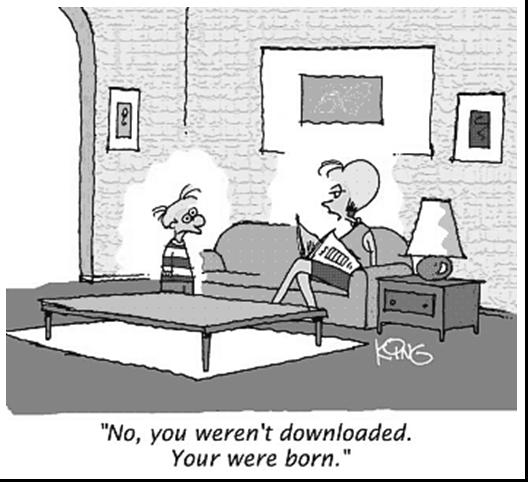
\includegraphics[width=0.4\textwidth]{fig1.jpg} % altere a width (intervalo entre 0.0 e 1), caso a imagem não fique na posição correta
        \caption{Exemplo de uso de figura}
        \label{fig:figura1}
    \end{figure}

    % Figuras (usando subfigure)
    % https://latex-tutorial.com/subfigure-latex/
    \begin{figure}[h!] % h! pede para o compilador tentar incluir a figura na posição em que foi declarada;
        \centering
        \caption{Exemplo com sub-figuras}
        \begin{subfigure}{0.4\textwidth}
            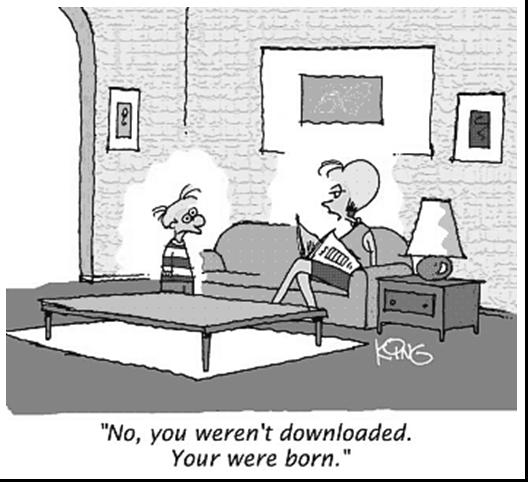
\includegraphics[width=\textwidth]{fig1.jpg}
            \caption{Sub-figura 1}
            \label{fig:sub_fig1}
        \end{subfigure}
        \hspace{1em}
        \begin{subfigure}{0.4\textwidth}
            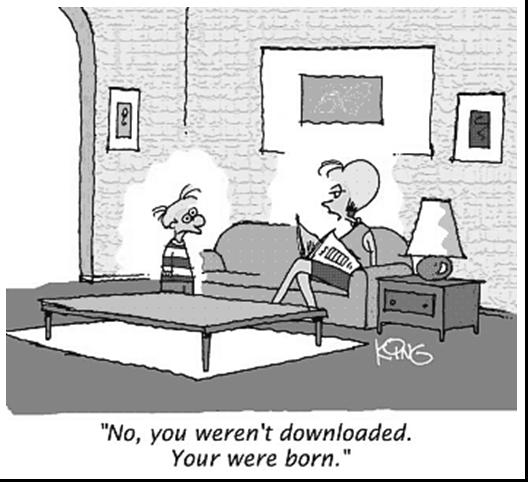
\includegraphics[width=\textwidth]{fig1.jpg}
            \caption{Sub-figura 2}
            \label{fig:sub_fig2}
        \end{subfigure}
        \label{fig:figura2}
    \end{figure}
    
    % Tabelas
    % Editor online: https://www.latex-tables.com
    % Referência: https://ctan.math.illinois.edu/macros/latex/contrib/tabularray/tabularray.pdf
     \begin{table}[H] % h! pede para o compilador tentar incluir a tabela na posição em que foi declarada;
        \centering
        \caption{Minha tabela}
        \label{tab:tabela1}
        \begin{tblr}{
          colspec = {X[l] X[l]}, % Tipo X define células com quebra automática de linha. Use: l=left, r=right, c=center ou j=justify para alinhamento dentro das células
          width = \linewidth,
          hlines, % inclui borda horizontal
          vlines, % inclui borda vertical        
        }
        \textbf{cabeçalho 1} & \textbf{cabeçalho 2} \\
        {texto à esquerda} & {Existem muitas variações das passagens do Lorem Ipsum disponíveis, mas a maior parte sofreu alterações de alguma forma.}
        \end{tblr}        
    \end{table}

    % tabela com subtabelas
    \begin{table}[H]
        \centering
        \caption{Tabela com sub-tabelas}
        \label{tab:tabela2}
        \begin{subtable}{0.45\linewidth} %subtabela
            \centering            
            \begin{tblr}{
              colspec = {X[l] X[l]}, % Tipo X define células com quebra automática de linha. Use: l=left, r=right, c=center ou j=justify para alinhamento dentro das células
              width = \linewidth,
              hlines, % inclui borda horizontal
              vlines, % inclui borda vertical        
            }
            \textbf{cabeçalho 1} & \textbf{cabeçalho 2} \\
            {Contrary to popular belief, Lorem Ipsum is not simply random text. It has roots in a piece of classical Latin literature from 45 BC, making it over 2000 years old.} & {The standard chunk of Lorem Ipsum used since the 1500s is reproduced below for those interested.}
            \end{tblr}
            \caption{Sub-tabela da esquerda}
        \end{subtable}
        \hfill
        \begin{subtable}{0.45\linewidth} %subtabela
            \centering            
            \begin{tblr}{
                  colspec = {X[l] X[l]}, % Tipo X define células com quebra automática de linha. Use: l=left, r=right, c=center ou j=justify para alinhamento dentro das células
                  width = \linewidth,
                  hlines, % inclui borda horizontal
                  vlines, % inclui borda vertical        
                }
                \textbf{cabeçalho 1} & \textbf{cabeçalho 2} \\
                {Contrary to popular belief, Lorem Ipsum is not simply random text. It has roots in a piece of classical Latin literature from 45 BC, making it over 2000 years old.} & {The standard chunk of Lorem Ipsum used since the 1500s is reproduced below for those interested.}
            \end{tblr}
            \caption{Sub-tabela da direita}
        \end{subtable}
    \end{table}

\section{Considerações Finais}
Essa seção deverá ser escrita na segunda parte do trabalho, conhecida como TCC2.

% %%%%%%%%%%%%%%%%%%%%%%%%%%%%%%%%%%%%%%%%%%%%%%%%%%%%%%%%%%%%%%
% Seção de Referências (gerada automaticamente)
\printbibliography  % Não remover esta linha
% %%%%%%%%%%%%%%%%%%%%%%%%%%%%%%%%%%%%%%%%%%%%%%%%%%%%%%%%%%%%%%

\end{document}